
\documentclass[conference]{IEEEtran}

\usepackage[utf8]{inputenc}	% arquivos LaTeX em Unicode (UTF8)
\RequirePackage[plainpages,pdfpagelabels]{hyperref}	% PDF com links, metadados


% *** GRAPHICS RELATED PACKAGES ***
%
\ifCLASSINFOpdf
  \usepackage[pdftex]{graphicx}
  \graphicspath{{../pdf/}{../jpeg/}{./plots/}}
  \DeclareGraphicsExtensions{.pdf,.jpeg,.png}
\else
\fi


\usepackage{cleveref}
\usepackage{subfig}

\usepackage{tikz}
\def\checkmark{\tikz\fill[scale=0.4](0,.35) -- (.25,0) -- (1,.7) -- (.25,.15) -- cycle;} 
\def\scalecheck{\resizebox{\widthof{\checkmark}*\ratio{\widthof{x}}{\widthof{\normalsize x}}}{!}{\checkmark}}

% *** SPECIALIZED LIST PACKAGES ***
%
\usepackage{algorithm}
\usepackage[noend]{algpseudocode}
\floatname{algorithm}{Algorithm}
\renewcommand{\algorithmiccomment}[1]{~~~// #1}

\hyphenation{op-tical net-works semi-conduc-tor}


\begin{document}

\title{TruMan: Trust Management for Vehicular Networks}


%\author{\IEEEauthorblockN{Renan Greca}
%\IEEEauthorblockA{Departamento de Informática\\
%Universidade Federal do Paraná\\
%Curitiba, Brazil\\
%Email: rdmgreca@inf.ufpr.br}
%\and
%\IEEEauthorblockN{Luiz Carlos P. Albini}
%\IEEEauthorblockA{Departamento de Informática\\
%Universidade Federal do Paraná\\
%Curitiba, Brazil\\
%Email: albini@inf.ufpr.br}}

\author{\IEEEauthorblockN{Renan Greca and Luiz Carlos Pessoa Albini}
        \IEEEauthorblockA{Department of Informatics -- Federal University of Paraná (UFPR) -- Curitiba, Brazil\\
                          Email: rdmgreca@inf.ufpr.br, albini@inf.ufpr.br}
}


\maketitle

\begin{abstract}
By integrating processors and wireless communication units into vehicles, it is possible to create a vehicular ad-hoc network (VANET), in which cars share data amongst themselves in order to cooperate and make roads safer and more efficient.
A decentralized ad-hoc solution, which does not rely on previously existing infrastructure, Internet connection or server availability, is preferred so the message delivery latency is as short as possible in the case of life-critical situations.
However, as it is the case with most new technologies, VANETs will be a prime target for attacks performed by malicious users, who may benefit from affecting traffic conditions.
In order to avoid such attacks, one important feature for vehicular networks is trust management, which allows nodes to filter incoming messages according to previously established trust values assigned to other nodes.
To generate these trust values, nodes use information acquired from past interactions. Nodes which frequently share false or irrelevant data must have lower trust values than the ones which appear to be reliable.
This work proposes a trust management model in the context of daily commutes, utilizing the Working Day Movement Model as a basis for node mobility.
The results prove to be accurate and efficient, thanks to the low complexity of the algorithm constituting the trust model.
\end{abstract}

%\begin{IEEEkeywords}
%Vehicular Network; Trust Management; V2V Communication;
%\end{IEEEkeywords}

\IEEEpeerreviewmaketitle



\section{Introduction}
\label{section:introduction}

Within the next few years, a substantial share of new vehicles will come equipped with networking features \cite{connectedcar2016}.
These features will allow vehicles to quickly share data with other nearby devices and can be useful tools to reduce traffic and the risk of accidents.
Over one million people lose their lives to traffic accidents every year \cite{whotraffic}, so solutions to improve road safety are crucial for modern life.
%Vehicular ad-hoc networks are a much-studied usage of vehicular networking features.
%In these networks, all nodes are related to traffic; they can be vehicles equipped with on-board computers, or stationary units placed near roads.
By quickly sharing data with neighboring vehicles without the need of an Internet connection, smart vehicles can alert drivers of important road conditions \cite{barba2012smart}, while autonomous vehicles can synchronize their movements to maximize traffic throughput \cite{amoozadeh2015platoon}.

The communication standard for vehicular communication is the IEEE 802.11p or Wireless Access in Vehicular Environments (WAVE) \cite{jiang2008ieee}.
It describes two types of nodes for vehicular networks: on-board units (OBUs) and road-side units (RSUs).
Communication between two OBUs is called vehicle-to-vehicle (V2V) communication, while communication between an OBU and an RSU is called vehicle-to-infrastructure (V2I) communication.
This study focuses only on V2V scenarios, and therefore, any references to Vehicular ad-hoc networks (VANETs) and their nodes refer exclusively to vehicles with on-board units.

As expected for new technologies, vehicular communications can become an appealing target for malicious users and attackers.
Some issues that could be exploited in such network include: vehicles with faulty sensors \cite{isaac2010security}; vehicles broadcasting false data \cite{golle2004detecting}; a flood of false data to generate a distributed denial of service (DDoS) scenario or to divert traffic \cite{garip2015congestion}; eavesdropping on other vehicles' communications, signal jamming or stalking \cite{isaac2010security}. 

Each of these problems require specific solutions, although there are ways of making the network safer in general.
One way is taking advantage of the concept of trust between network members.
By having nodes remembering previous interactions with one another, it is possible for them to build trust relationships and avoid those attacks that involve the spread of false data.
Trust solutions for VANETs are generally classified into data-oriented, emphasizing the message contents, or entity-based, emphasizing message senders.

This work proposes a new and improved entity-based trust model to compute the trust between any pair of nodes in a vehicular network.
Using the proposed trust model, nodes in a vehicular network are able to identify which other nodes are likely malicious.
Since the network is dynamic, nodes acquire more knowledge as time passes and the results of the algorithm become more precise, taking advantage of social properties of VANETs \cite{da2013effective} \cite{cunha2014possible} to build strong relationships between frequently connected nodes.
Simulations demonstrate that nodes are able to correctly identify more than 95\% of nodes in the network (malicious or not).
The algorithm correctness depends upon the velocity of the nodes, the frequency of the information exchanged between them and the running time, i.e. the longevity, of the algorithm.
%After running a series of simulations, the results were very promising; after one simulated day, 

%==> O QUE SE PRETENDE ATINGIR? O QUE TEM DE DIFERENTE? QUAIS RESULTADOS FORAM OBTIDOS? FALTA UM PARAGRAFO AQUI FALANDO DISSO.

The remainder of this paper is organized as follows.
Section \ref{section:algorithm} details the proposed trust model;
Section \ref{section:results} contains the simulation results which demonstrate the usefulness of the model;
Section \ref{section:previouswork} presents the previously published trust models for vehicular networks and compares them with TruMan;
and Section \ref{section:conclusion} has the conclusion and future work directions.

\section{TruMan}
\label{section:algorithm}

%==> MUDAR O TITULO, PRACISA DIZER ALGO DO TIPO UNDERNEATH ALGORITHM

The objective of the TruMan trust model is to allow nodes to infer whether or not other nodes in the network are malicious.
The algorithm that dictates the trust model runs continuously, with iterations happening in preset intervals.
In every iteration, a node collects information from its neighbors and runs a combination of algorithms to detect malicious nodes in the known network.
This information is maintained in a directed graph $T=(V,E)$, in which $V$ is the set of known vertices and $E$ is the set of known trust relationships between pairs $u,v \in V$.
Graph $T$ is known as the \textit{trust graph}.

Each edge $(u, v) \in E$ stores a value between 0 and 1 which represents the degree of trust $u$ has for $v$.
This value is called the \textit{opinion} of $u$ about $v$.
At the start of the execution, edges have value $0.5$; this value increases when nodes have positive interactions and decreases otherwise.
A threshold $0 < h < 1$ is used to define the minimum weight for an edge to be considered positive, meaning that the origin node trusts the destination node.
%By default, the threshold is $0.5$.

After collecting information from other nodes, TruMan performs two steps: ($i$) it divides the network graph into strongly connected components using Tarjan's algorithm; ($ii$) it uses a graph coloring algorithm as a heuristic to determine which nodes to trust or not.

%In order to do this, a node must maintain a graph $T=(V,O)$ that represents its knowledge of the network, in which $V$ is the set of known nodes and $O$ is the set of opinions nodes have about others.
%Opinions are directed edges, each one with a weight between 0 and 1 that represents the degree of trust from one node towards another.
%A threshold $0 < h < 1$ may be used as a parameter to define the minimum weight for an edge to be considered positive, meaning that the origin node trusts the destination node.


The detailed descriptions of both algorithms are below, followed by the complete process of each iteration of the Truman trust model.


%==> VOCE AINDA NAO FALOU DOS PESOS DAS ARESTAS E COMO ELES FORAM CONSEGUIDOS
%==> VOCE NAO FALOU DOS GRAFOS

% ---------------------------------------------------------------------------------------------------
\subsection{Tarjan's strongly connected components algorithm}
\label{section:tarjan}
The use of Tarjan's strongly connected components algorithm \cite{tarjan1972depth} is an important aspect of TruMan's efficiency.
This allows a large graph to be abstracted into a smaller one, which therefore reduces the input for further steps.
Given a directed graph $T = (V,E)$, a strongly connected component is defined as a group of nodes in which, for any pair of nodes $u, v \in V$, there is a path from $u$ to $v$ and a path from $v$ to $u$.
For the purposes of trust management, this definition is extended to accept only paths of edges with weight above a predetermined threshold $h$.
Every node of the input graph $T$ must belong to a component.


%-----ACHO QUE ESTA DEFINIÇAO ESTA COM MUITOS DETALHES DE IMPLEMENTACAO ---
%-----PODERIA DEIXAR ELA MAIS ALTO NIVEL, EM FORMA DE CONJUNTOS POR EXEMPLO ---


%Three data structures are used by the algorithm:
%$index$ and $lowlink$ are indexed by node IDs (predefined unique identifiers) and $stack$ is a last-in-first-out stack.
%The $count$ variable is incremented at each visited node.
%In the implementation used, $index$, $lowlink$, $count$ and $stack$ are global variables accessible from every call of the function.
%$index$ and $lowlink$ are arrays indexed by node IDs (predefined unique identifiers), $count$ is an integer and $stack$ is a last-in-first-out data structure.

%The algorithm works by performing a depth-first search, adding nodes to a stack as they are visited.
%If two nodes are present on the stack, then there is a path from the first node to the second one (in the order they were added to the stack).
%Each node has two attributes assigned to it during the execution of the algorithm: $index$ is used to number the nodes in the order they are visited, while $lowlink$ is the lowest indexed node reachable from each node.
%
%In the call that visits a node $u$, the algorithm must loop through each node $v$ trusted by $u$ (that is, $u \rightarrow v$ exists and has value greater than $h$).
%If node $v$ has not yet been visited, the algorithm is called for  $v$.
%The $lowlink$ of $u$ is then calculated as the smallest value between $lowlink[u]$ and $lowlink[v]$, because any node reachable from $v$ is also reachable from $u$.
%After the loop, if $lowlink[u]$ is equal to $index[u]$, it means that $u$ is the lowest indexed node reachable from itself and that it is the root of a component.
%Therefore, nodes must be popped from the stack until $u$ is found.
%Each node popped, including $u$, is a member of a strongly connected component.

%---------------

The number of components is, at most, $|V|$: in a worst-case scenario, each node is placed into its own component.
The complexity of the algorithm is $O(|V|+|E|)$ for a graph $T = (V,E)$.
%; however, this would not be the case for most useful input graphs.   ---> NÃO ENTENDI <---

%Algorithm \autoref{algorithm:tarjan} shows the general structure of Tarjan's algorithm  \cite{tarjan1972depth}.

From the output of Tarjan's algorithm, an undirected component graph $C = (V',E')$ is formed.
Each $v' \in V'$ is the abstraction of one component identified by Tarjan's algorithm, while the edges $e' \in E'$ are edges from $T$ between nodes that do not belong in the same component (e.g. if $u$ and $v$ are separated into $u'$ and $v'$, $e = (u,v)$ becomes $e'=(u',v')$.

%\begin{algorithm}
%\caption{Tarjan's strongly connected components algorithm}\label{algorithm:tarjan}
%\begin{algorithmic}[1]
%
%\Function{Tarjan}{vertex $u$}
%
%\State $index[u] = count$
%\State $lowlink[u] = count$
%\State $count \gets count + 1$
%\State \textbf{push} $u$ \textbf{to} $stack$
%
%\For{$v$ \textbf{in} neighbors of $u$ }
%	\If{weight of $u \rightarrow v$ $<$ $h$}
%		\State \textbf{continue}
%	\EndIf	
%		
%	\If{$index[v] = -1$}
%		\Comment{\emph{v has not been visited yet}}
%		\State \textbf{Tarjan}($v$)
%	\EndIf
%	
%	\State $lowlink[u] \gets \textbf{min}(lowlink[u],lowlink[v])$
%\EndFor
%
%\If{$lowlink[u] = index[u]$}
%	\Repeat
%		\Comment{\emph{unstack nodes until u is found}}
%		\State \textbf{pop} $w$ \textbf{from} $stack$
%		\State \textbf{add} $w$ \textbf{to} $component$
%	\Until {$w = u$}
%\EndIf
%
%\EndFunction
%\end{algorithmic}
%\end{algorithm}

% ---------------------------------------------------------------------------------------------------
\subsection{Graph coloring with minimum colors}
\label{section:coloring}
The algorithm proposed in \cite{mittal2011graph} is an efficient approach to graph coloring.
Graph coloring is one of the possible heuristics used to detect malicious nodes after the generation of the component graph using Tarjan's algorithm.
Out of the tested heuristics, it presents the best results, so it has been chosen as the heuristic for the trust model.

%The process of graph coloring consists of labeling each node with a color so that no two neighboring nodes share the same color.
%This problem has been studied in Computer Science since, at least, 1972 \cite{karp1972reducibility} and has been studied as a classic mathematics problem for even longer \cite{kempe1879geographical}.
It has been mathematically proven that any planar graph can be colored with at most four colors \cite{appel1976every}, but discovering the smallest number of colors necessary to color an arbitrary graph (called the chromatic number of the graph) is an NP-hard problem \cite{sanchez1989determining}.
In \cite{mittal2011graph}, the authors propose to color a graph using the minimum possible amount of colors.
Although they do not prove that their algorithm always uses the smallest possible amount of colors, the output is always a correct coloration and the algorithm is nevertheless efficient.
The complexity of the algorithm is $O(|E'|)$ for a graph $C = (V',E')$.
As a comparison, the classic DSATUR algorithm for graph coloring has complexity $O(|V'|^2)$ \cite{brelaz1979new}.
%For the purposes of this study, it is not necessary to prove that the coloring algorithm's output uses the minimum possible number of colors.

%Algorithm \autoref{algorithm:coloring} shows the general structure of the graph coloring algorithm  \cite{mittal2011graph}.
%
%A limitation of this algorithm is that the edges must be sorted according to node indexes beforehand.
%It does not matter which nodes get assigned which indexes, but once they are assigned those numbers, the algorithm must follow the edges in numerical order.
%This is demonstrated in \cite{vernize2013dissertation}.

%\begin{algorithm}
%\caption{Graph coloring with minimum colors}\label{algorithm:coloring}
%\begin{algorithmic}[1]
%
%\Function{Coloring}{graph $G$}
%
%\State \textbf{color} all nodes of $G$ \textbf{with} 0
%\State $d \rightarrow 0$
%\For{$e=(u,v)$ \textbf{in} edges of $G$}
%	\If{$u$ and $v$ have the same color}
%		\If{$color[v] = d$}
%			\State $d \rightarrow d+1$
%		\EndIf
%		\State $color[v] \rightarrow d$
%	\EndIf
%\EndFor
%
%
%\EndFunction
%\end{algorithmic}
%\end{algorithm}

% ---------------------------------------------------------------------------------------------------
\subsection{The TruMan algorithm}
\label{section:trustmanagement}
%\subsection{Malicious Node Identification Algorithm}
%\label{section:mani}

%The basis of the presented trust model is the Malicious Node Identification Algorithm (MaNI) proposed in \cite{vernize2015malicious}, \cite{vernize2013dissertation}.
%The authors present a malicious node identification scheme based on strongly connected components and graph coloring.
%The model is proposed for complex networks in general, but is not suited for VANETs because it is designed only for static networks.
%Furthermore, the algorithm is executed by a global observer which has information about the complete network.


%==> ALGUMAS PARTES ESTÃO MUITO REPETITIVAS COM A SEÇAO DE CIMA. PRECISA REVER PARA NÃO FICAR MUITO REPETITIVO. <==


TruMan is based on the MaNI algorithm \cite{vernize2015malicious}, which suggested the use of Tarjan's algorithm and the graph coloring algorithm.
However, MaNI was developed for static networks such as social networks, and is executed by an external supervising agent (i.e. outside of the network), making it unsuitable for a vehicular network.
%The work describes here takes advantage of the efficiency of the two graph theory algorithms into a model that is viable for highly dynamic networks.

%In order to work with dynamic networks, the Truman algorithm must consider snapshots as inputs.
%The algorithm runs continuously, running new iterations at predetermined intervals.
%Each iteration $i$ is associated with a timestamp, which indicates when the snapshot was taken.
%A snapshot $S_i$ represents the complete topology of the network at the iteration $i$.
%%; $V_i$ is the set of nodes participating in the network at that time and $E_i$ is the set of edges connecting pairs of nodes within communication range of each other.
%As the network is dynamic, it is expected that each $S_i$ is different from $S_{i-1}$, but also that the changes follow a determined mobility model.

In order to work with dynamic networks, the TruMan algorithm runs iterations at predetermined intervals.
%As nodes acquire more information, their model of the network will change.
Furthermore, the algorithm runs in a decentralized fashion, meaning each node in the network runs its own instance of the algorithm.
Each node starts knowing information only about itself and maintains its own abstraction of the network surrounding it.
Every node $u$ stores a representation of the network in the form of a static, connected and directed trust graph $T = (V, E)$, in which $V$ is the set of nodes node $u$ is aware of and $E$ is the set of trust relationships (opinions) $u$ knows between members of $V$.
Since each node has its own network representation and it changes over time, there is a $T^u_i = (V^u_i, E^u_i)$ for every node $u$ and iteration $i$.

%==> VOCE NAO FALOU DOS PESOS DAS ARESTAS AINDA

%==> ACHO QUE PRECISA FALAR AQUI DA PRINCIPAL DIFERENCA PARA O MaNI, QUE AQUI ESTAMOS FALANDO DE REDE MOVEL E ALGORITMO DISTRIBUIDO

At first, the node collects and organizes information.
A prerequisite of this step is a test that correctly classifies a neighboring node as benign or malicious.
There are several ways to perform such a test, but a study between these methods is beyond the scope of this paper.
Every time a neighboring node $v$ is tested as benign, the value of $u \rightarrow v$ increases and the trust graph $T^v_{i-1}$ is merged into $u$'s trust graph.
After this, a new $T^u_i$ is formed, which is used for the remaining steps.

%Each edge $w \rightarrow v \in E^u_i$ is weighted according to the degree of trust $w$ has for $v$ with a value between 0 and 1.
%The closer the value is to 1, the more $w$ trusts $v$.
%These values are not mutual, so the value of $w \rightarrow v$ can be different from the value of $v \rightarrow w$.

After the collection of data, $T^u_i$ is separated into strongly connected components using Tarjan's algorithm \cite{tarjan1972depth}.
For each node in a component, there is a path formed by edges of weight higher than the threshold $h$ to each other node in the same component.
In other words, within a single component, all nodes trust one another directly or indirectly; nodes that do not satisfy this condition are separated into different components.
Each of these components becomes a node of a component graph $C^u_i = (V'^u_i, E'^u_i)$.

The creation of $C^u_i$ simplifies the remaining computation.
Since each vertex $v' \in V'^u_i$ is a component of $T^u_i$ in which all nodes trust each other, for the purposes of identifying malicious nodes, all nodes within each of those components can be treated as the same.
They can either be benign nodes which legitimately trust one another, or malicious nodes colluding with each other.
After the formation of $C^u_i$, a heuristic is used to classify the nodes as benign or malicious.


%==> PRIMEIRA FRASE ESTA ESTRANHA <==
The coloring heuristic is used to classify nodes, which uses the algorithm described in \autoref{section:coloring} \cite{mittal2011graph}, although other heuristics may be considered.
After running the graph coloring algorithm with graph $C^u_i$ as input, the color whose nodes in $C^u_i$ represent the most nodes in $T^u_i$ is classified as correct, and all others are classified as malicious.
Once this information from $C^u_i$ is brought back to graph $T^u_i$, it is trivial to label the nodes in $T^u_i$ as either benign or malicious based on the classifications of their components.

%In the experiments shown in \cite{vernize2013dissertation}, the coloring heuristic shows the most promising results, identifying a high ratio of the malicious nodes in the network.
%Other heuristics were experimented with, but were either less effective in detecting malicious nodes, or provided too many false positives.
%Therefore, for the purposes of this research, only the coloring heuristic is considered.

The complexity of the whole algorithm can be calculated by adding the most costly operations involved.
As discussed above, Tarjan's algorithm has a complexity of $O(|V|+|E|)$ (for the trust graph $T$), while the graph coloring algorithm has a complexity of $O(|E'|)$ (for the component graph $C$).
The most costly part of the algorithm is the graph merge operation that happens between trusted nodes.
The complexity of the graph merge algorithm is $O(|E|)$ for each neighbor a node has in an iteration; this number is at most $|V|$.
The total complexity of TruMan is, therefore, $O(|V|+|E|)+O(|E'|)+O(|V|\times |E|)$.
Since $|E'| \leq |E|$ and $|V|+|E| \leq |V|\times |E|$, the complexity can be simplified to $O(|V| \times |E|)$.

In summary, every node $u$ runs the following steps in each iteration to detect malicious nodes in the network:

\begin{enumerate}
	\item Node $u$ checks which are its neighbors (nodes within its communication range).
		  New discovered nodes and new formed edges are added to $T^u_i$.
		  Edges are created with weight 0.5.
	\item Node $u$ tests all its neighbors to discover which ones can be directly trusted or not.
		  New trust values are computed for the edges using the average between the previous value and either 1 (if the neighbor is trustworthy) or 0 (otherwise).
	\item If a neighbor $v$ is trustworthy, $u$ merges $T^v_{i-1}$ into $T^u_i$.
	\item Tarjan's algorithm is executed to identify the strongly connected components of $T^u_i$, resulting in a component graph $C^u_i$.
	\item The graph coloring algorithm is executed on $C^u_i$ and nodes are classified as benign or malicious. %according to the same rules as the MaNI algorithm.
\end{enumerate}

%Two types of experiments were made in each network: first, all malicious nodes inverted the edge weights leading to their neighbors; second, malicious nodes randomly inverted or not the weights.
%In the first scenario, the results show excellent precision in most networks, detecting nearly every malicious node.
%Experimenting with the second scenario, the results are less precise, however still promising: with up to 20\% of malicious nodes in the network, the error rate is under 7\%, while with the worst case, 50\% of the network being malicious, the error rate is approximately 15\%.
%
%The authors suggest running the algorithm repeatedly after removing the malicious nodes from the network.
%By doing this, nearly all malicious nodes are detected by it even when randomly changing edge weights.


% ---------------------------------------------------------------------------------------------------

%The MaNI algorithm works well and is efficient for static graphs.
%However, some important modifications had to be made to accommodate dynamic graphs in a decentralized fashion.
%The main changes made are described below.

%First of all, 


%Another important change is on the trust values themselves.
%MaNI uses binary trust (either 0 or 1).
%This has been replaced by a floating-point number between 0 and 1; a predefined threshold defines which values are deemed trustworthy or not.
%This was not the case in the first versions of the trust model; it was added in order to avoid abrupt changes to opinions.
%Since the network is different on each iteration of the algorithm, there were instances in which a change to the topology caused a radical change to the output of the graph coloring algorithm.
%Using a trust value that gradually changes over time, output variations between two iterations became small and gradual.
%
%At the start of an execution, a node knows only about itself.
%From that point, iterations of the algorithm will run in a set interval of $l$ seconds.
%In each iteration (labeled $t$ after the timestamp it occurs on) and for every node $u$, the following steps are executed:





%To mention:
%- Graph building;
%- Change from binary trust to a weighted model;
%- Evolution of trust over time.

%First of all, there is an important change to the graph knowledge used to run the algorithm.
%The complete trust graph is a parameter to the MaNI algorithm, which is executed by a supervisor with global knowledge of the graph.
%
%In this case, given a complete trust graph $T = (V, O)$, each node $u \in V$ has its own vision of the network and has to build a graph, called $T_u$, to represent its surrounding network.
%In each iteration of the algorithm, $u$ receives information from its neighbors about their own graphs.
%For every neighbor $v \in V$, $T_u$ must me merged with $T_v$.
%An edge $u \rightarrow v$ exists if $u$ is aware of $v$.
%Given sufficient iterations, $T_u$ forms a complete or nearly complete vision of the network.

%Alongside $G$, there is the trust graph $T = (V, O)$ which stores trust relationships between pairs of nodes in the form of directed edges.
%Again, each node $u$ has its own $T_u$, which contains the trust information node $u$ knows about.
%When a node $u$ asks for network information from node $v$, it also merges $T_u$ with $T_v$, but only if $u$ trusts $v$.
%If $u$ deems $v$ malicious, any information originating from $v$ cannot be considered valid.


%Furthermore, this implies that the malicious node detection algorithm runs using incomplete graph knowledge.
%This is expected and generally unavoidable in vehicular networks, which have high mobility and can be extremely large.

\section{Results}
\label{section:results}

In order to test the TruMan trust model, simulations were made using an implementation of the algorithm in Python.
To generate the input graphs with node mobility, the ONE simulator \cite{keranen2009one} was used in conjunction with the Working Day Movement Model \cite{ekman2008working}, which provides a strong similarity with vehicle movement in real life.
Snapshots of the network were taken every 10 simulated seconds, and these snapshots were used as input for the algorithm.

\begin{table}[h!]
\caption{Simulation parameters}
\label{table:parameters}
\centering
\begin{tabular}{|p{3cm}||p{3.5cm}|}
 \hline
 \textbf{Parameter}	& \textbf{Value} \\
 \hline
 \hline
 Duration 			& 86400 seconds \\
 \hline
 Work day length 	& 28800 seconds \\
 \hline
 Std. dev. departure time & 7200 seconds \\
 \hline
 Node velocity 		& 7~10m/s \\
 \hline
 Simulation area	& approximately 14km\textsuperscript{2} \\
 \hline
 Number of nodes 	& 150 (WDMM) + 10 (random) \\
 \hline
% Cost & O(|V|* |E|) & O(|V|+|E|) & n/a & n/a & n/a \\
% \hline
\end{tabular}
\end{table}

Most of the parameters for the simulator were taken from the article detailing the Working Day Movement Model \cite{ekman2008working}.
Different parameters are shown in \autoref{table:parameters}.
%The simulation ran for 86400 seconds (24 hours), with a work day length of 28800 seconds and a standard deviation of departure time of 7200 seconds.
%Nodes move between 7 and 10 m/s in an area of approximately 14 km\textsuperscript{2} based on a section of the map of Helsinki.
%%The number of nodes and their communication range vary for different simulations.
%There is a total of 160 nodes, 150 of which are following the Working Day Movement Model, and the other 10 are moving randomly to simulate vehicles that do not follow daily patterns.
Since this simulation is for vehicles instead of pedestrians, there are no buses in the model and every node is guaranteed to own a vehicle and travel by car.
The parameters regarding offices, meeting spots and shopping were kept intact.
A small part of nodes move randomly to simulate vehicles that do not follow daily patterns.

\subsection{Network Density}

%==> PRECISA MOSTRAR A EQUAÇÃO DE CALCULO DA DENSIDADE, SENÃO FICA DIFICIL DE ENTENDER O CALCULO.

The communication range of nodes varies from 10m to 50m, to illustrate the impact of different network densities.
The network density ($\delta$) is a value which abstracts the volume and frequency of connections in a vehicular network by estimating how much of the environment is covered by the network.
For TruMan, higher densities yield better results, since nodes can construct and update their models of the network faster (this is demonstrated in \autoref{subsection:simulations}).
It is calculated using the transmission range of the nodes ($\rho$), the amount of nodes ($\eta$), and the total area of the simulation ($\alpha$).

The coverage of a single node is the circumference around it formed by the transmission radius. This is divided by two to compensate for overlapping circumferences, then multiplied by the number of nodes in the network to estimate the maximum coverage area.
Finally, the value is divided by the total area of the environment.
The network density formula is as follows:

$$ \delta = \frac{\frac{\rho^2\pi}{2} \times \eta}{\alpha} $$

Simulations shown here have densities between 0.001 ($\rho = 10$m) and 0.04 ($\rho = 50$m).
As a comparison, the density of the city of São Paulo (Brazil) was calculated as 2.24 with $\rho = 10$m, a much higher value than what is necessary for a satisfactory performance of the algorithm.

\begin{figure*}[!t]
\centering
\subfloat[]{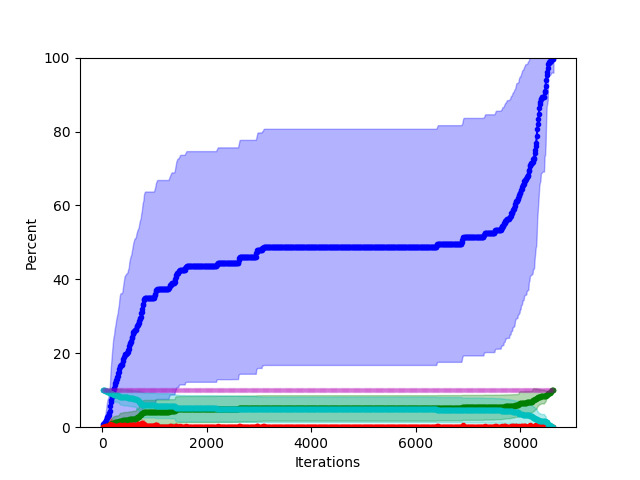
\includegraphics[width=0.329\linewidth]{Network_rA_10.0/new_plots/10.png}%
\label{subfig:random10}}
\hfil
\subfloat[]{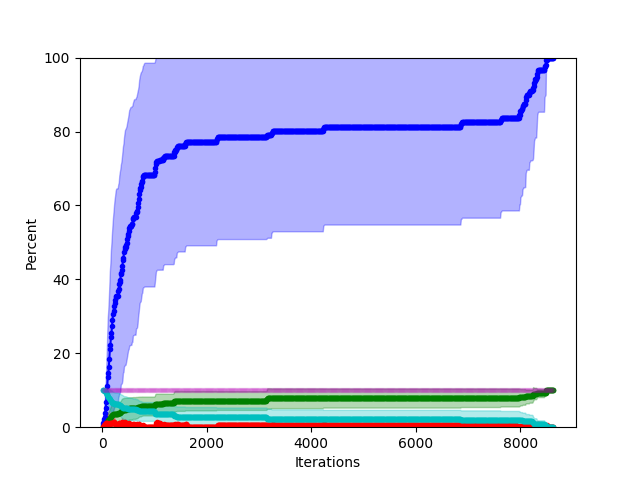
\includegraphics[width=0.329\linewidth]{Network_rA_10.0/new_plots/30.png}%
\label{subfig:random30}}
\hfil
\subfloat[]{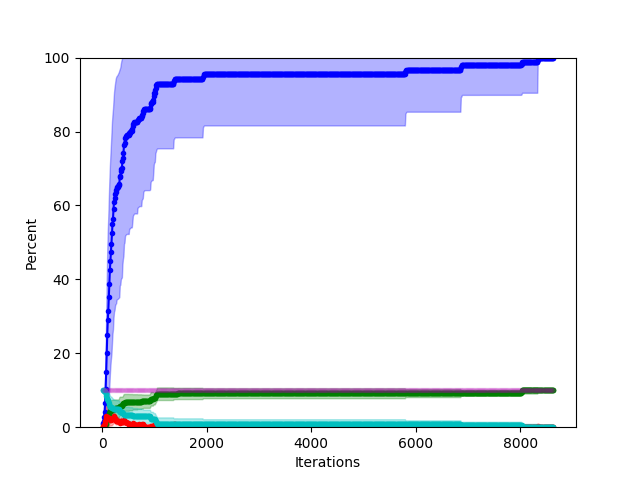
\includegraphics[width=0.329\linewidth]{Network_rA_10.0/new_plots/50.png}%
\label{subfig:random50}}
\caption{Simulation with 10\% malicious nodes and $\rho$ = (a) 10m, (b) 30m or (c) 50m.}
\label{fig:random103050}
\end{figure*}

\begin{figure*}[!t]
\centering
\subfloat[]{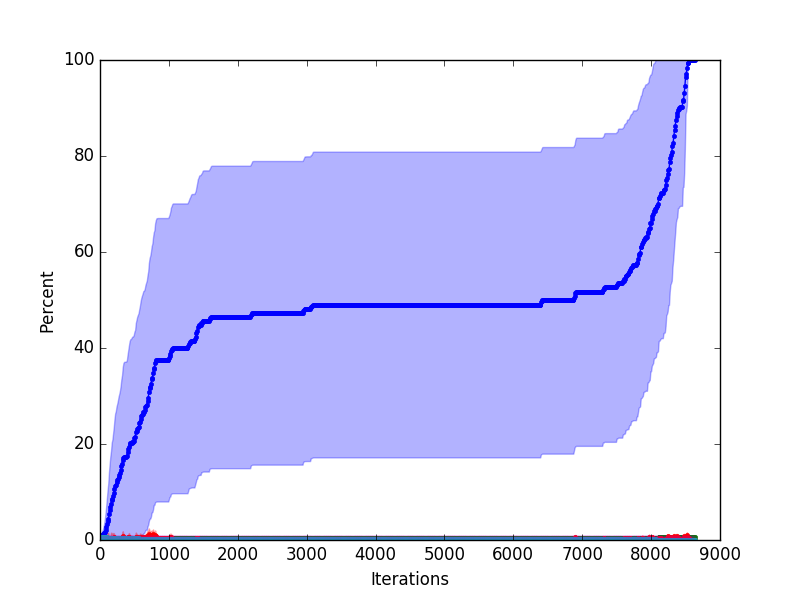
\includegraphics[width=0.329\linewidth]{Network_rA/10_1}%
\label{subfig:random1}}
\hfil
\subfloat[]{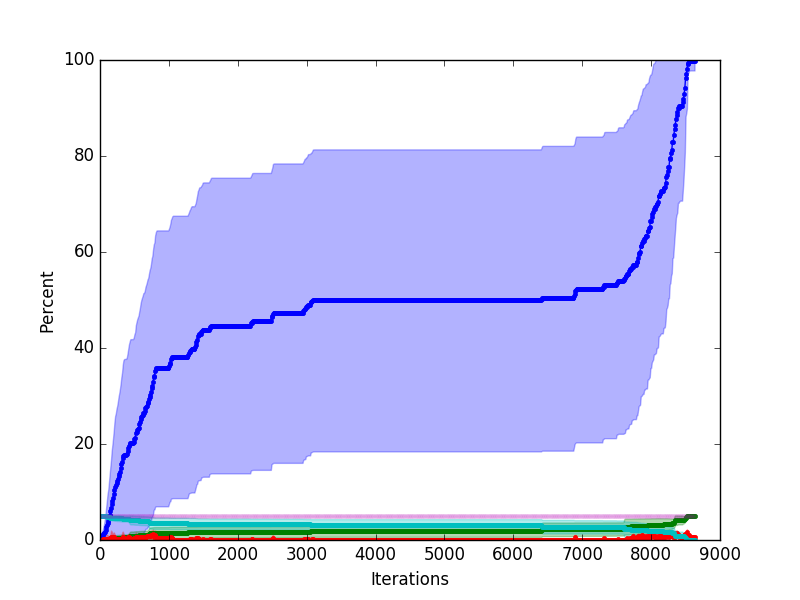
\includegraphics[width=0.329\linewidth]{Network_rA/10_5}%
\label{subfig:random2}}
\hfil
\subfloat[]{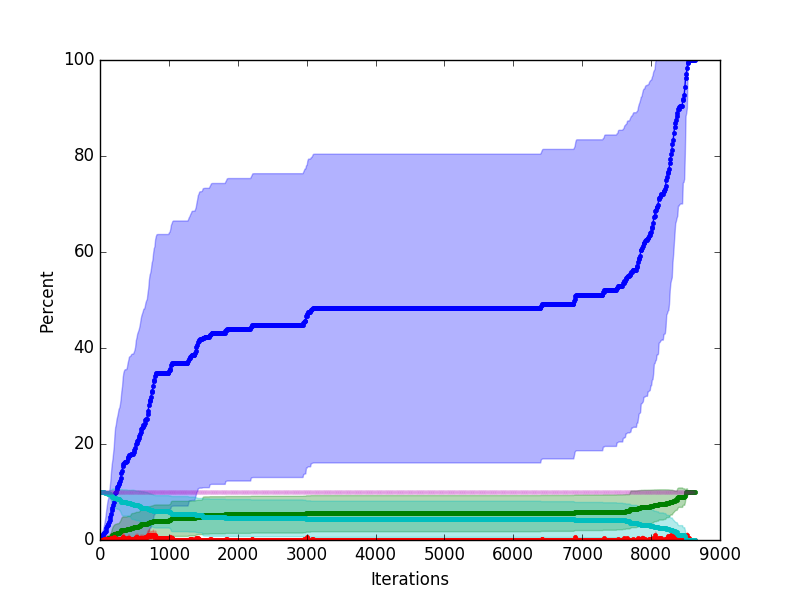
\includegraphics[width=0.329\linewidth]{Network_rA/10_10}%
\label{subfig:random3}}

\subfloat[]{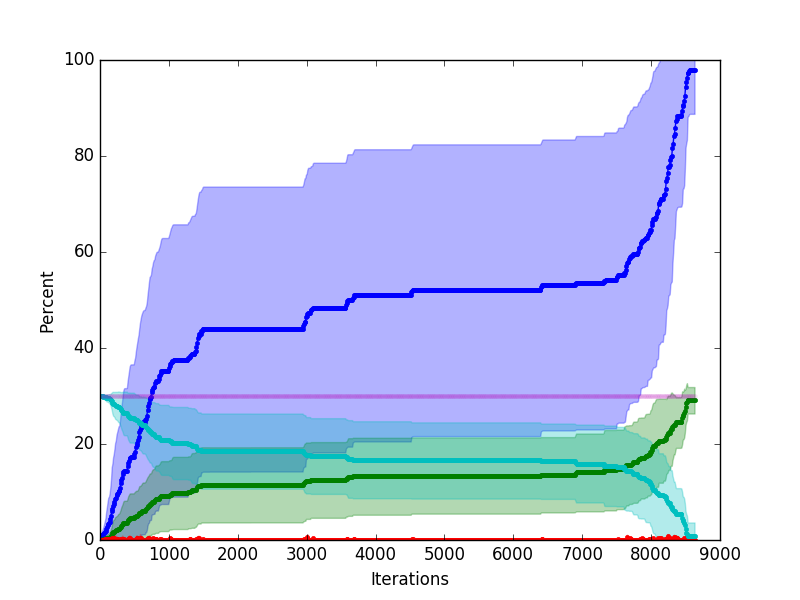
\includegraphics[width=0.329\linewidth]{Network_rA/10_30}%
\label{subfig:random4}}
\hfil
\subfloat[]{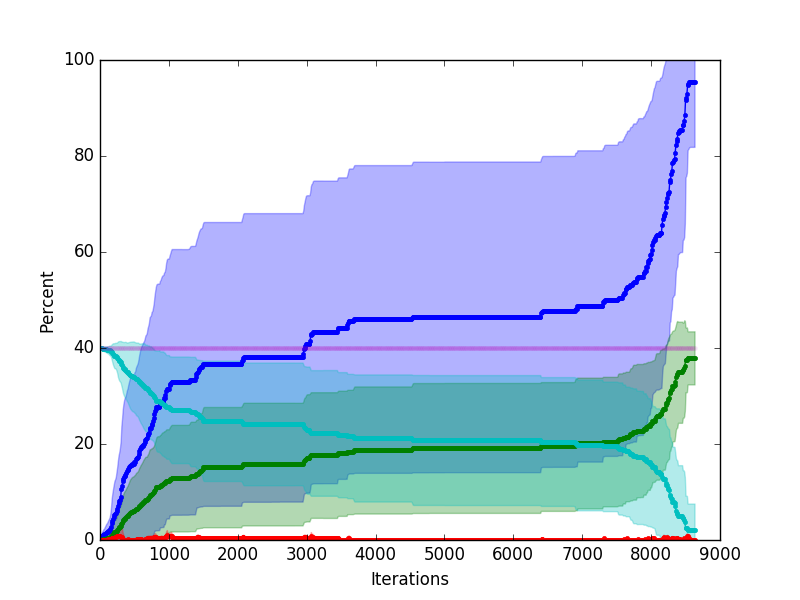
\includegraphics[width=0.329\linewidth]{Network_rA/10_40}%
\label{subfig:random5}}
\hfil
\subfloat[]{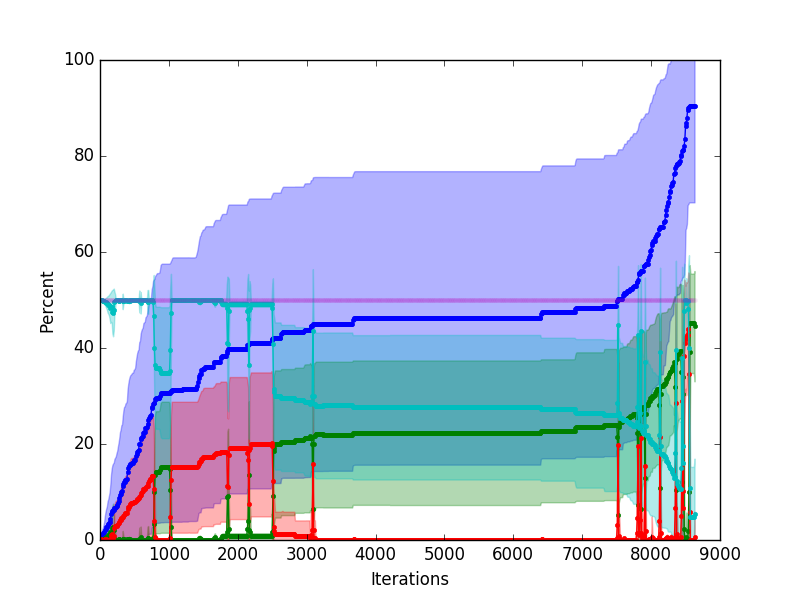
\includegraphics[width=0.329\linewidth]{Network_rA/10_50}%
\label{subfig:random6}}

\caption{Simulation with $\rho$ = 10m and (a) 1\%, (b) 5\%, (c) 10\%, (d) 30\%, (e) 40\% or (f) 50\% malicious.}
\label{fig:random0}
\end{figure*}

\subsection{Simulations}
\label{subsection:simulations}
To improve readability, all figures in this section follow the same format:
$X$ axis shows the results of sequential iterations, ranging from 0 to 8639;
$Y$ axis shows a percentage of all nodes in the network, ranging from 0 to 100;
blue line represents the percentage of nodes detected out of the complete network;
magenta is the percentage of malicious nodes in the network (ground truth);
green represents the nodes correctly identified as malicious (true positives);
cyan represents the undetected malicious nodes (false negatives); 
red represents the benign nodes incorrectly identified as malicious (false positives).

\autoref{fig:random103050} shows the results of simulations running with 10\% of nodes acting maliciously, with communications range varying from 10m to 50m.
It is possible to see how the increase in the range allows the algorithm to converge sooner, taking over 8000 iterations with 10m range and achieving solid results at just over 1000 iterations with 50m range. 

\autoref{fig:random0} shows the variation of results for different amounts of malicious nodes in the network.
By the end of one day, the algorithm is able to detect all malicious nodes when they are up to 30\% of the network.
At 40\%, a small part of malicious nodes are yet to be detected.
At 50\%, as expected, the results are inconsistent as the network is completely split between benign and malicious nodes; at this point, the network is completely compromised.
The amount of malicious nodes also affects the convergence of the algorithm, since nodes do not trust information from malicious neighbors.

\autoref{fig:random7} shows the execution of the algorithm over the course of 7 days.
Most malicious nodes are identified by the end of the first day; in the following iterations, the algorithm finishes building the network model and sorts out remaining false negative or false positive results.
After iteration 20000, the results are completely consistent.


%==> ACHO QUE PODIA USAR O MULTIFIGURE PARA AGRUPAR UM POUCO AS FIGURAS. COLOCA 3 LADO A LADO. ASSIM SOBRE ESPAÇO NO FINAL PARA PODERMOS COMPARAR COM TRABALHOS RELACIONADOS.

% ----
%
%\begin{figure}
%\centering
%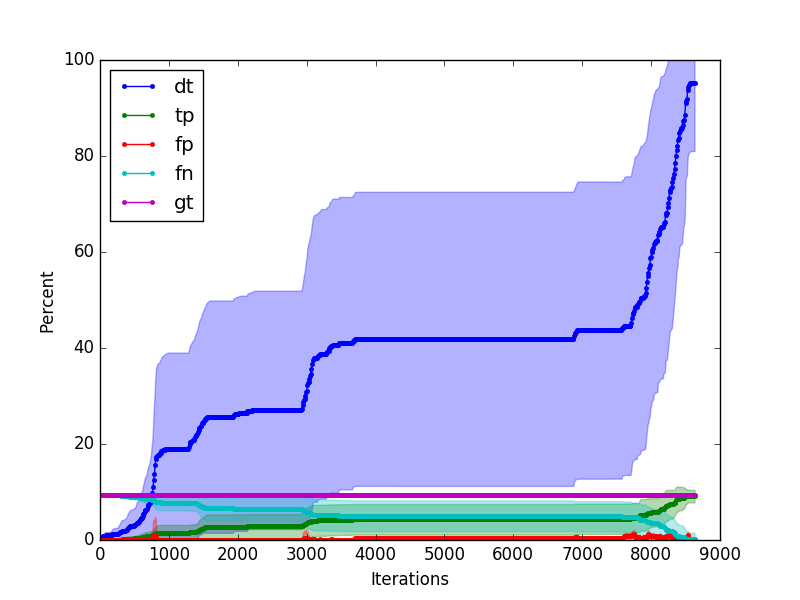
\includegraphics[width=0.5\lin0.5ewidth]{Network_A_10.0/new_plots/10.png}
%%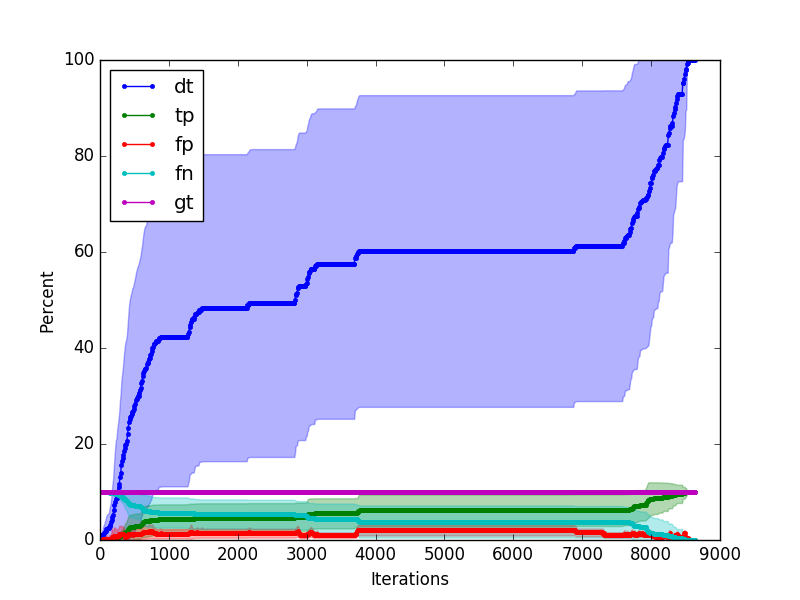
\includegraphics[width=0.45\linewidth]{Network_A_10.0/new_plots/30.png}
%\caption{Simulation without random nodes and range of 10m.} \label{fig:nonrandom1}
%\end{figure}
%
%\begin{figure}
%\centering
%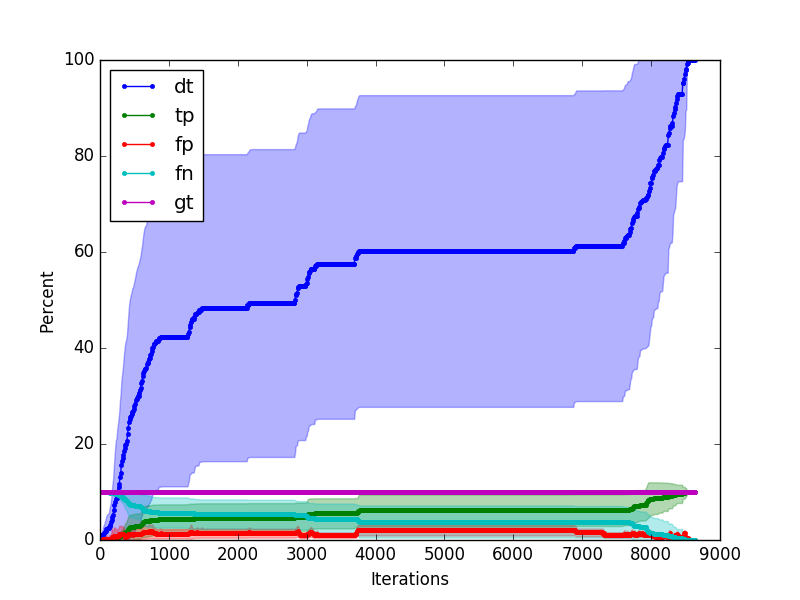
\includegraphics[width=0.5\linewidth]{Network_A_10.0/new_plots/30.png}
%\caption{Simulation without random nodes and range of 30m.} \label{fig:nonrandom2}
%\end{figure}
%
%\begin{figure}
%\centering
%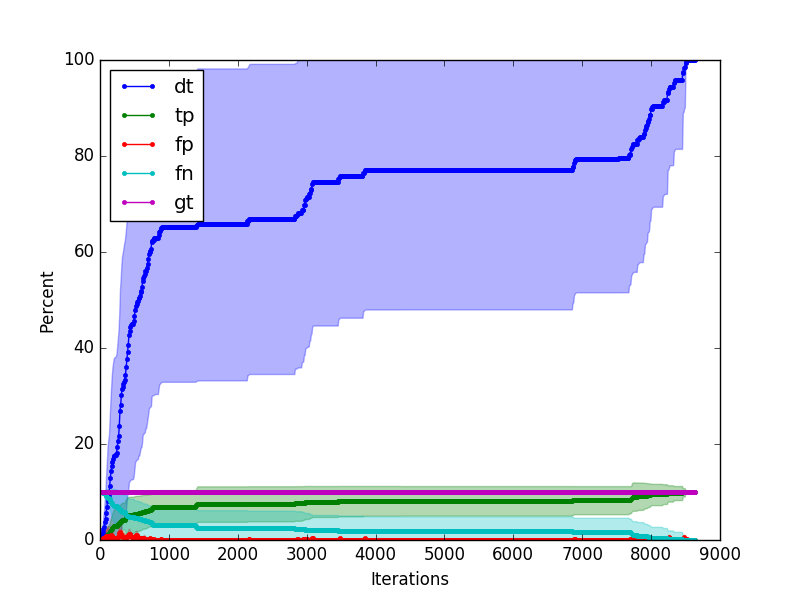
\includegraphics[width=0.5\linewidth]{Network_A_10.0/new_plots/50.png}
%\caption{Simulation without random nodes and range of 50m.} \label{fig:nonrandom3}
%\end{figure}

% ----


%==> AUMETEI UM POUCO AS FIGURAS, MAS ELAS PARECEM ESTAR MEIO DEFOCADAS, VE SE CONSEGUE MELHORAR UM POUCO A QUALIDADE DELAS.




%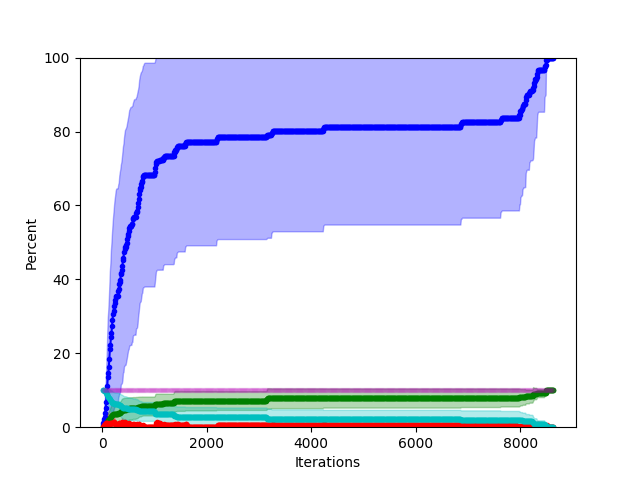
\includegraphics[width=0.329\linewidth]{Network_rA_10.0/new_plots/30.png}
%\caption{a}
%%\caption{Simulation with random nodes and range of 30m.} \label{fig:random30}
%%\hspace{1pt}
%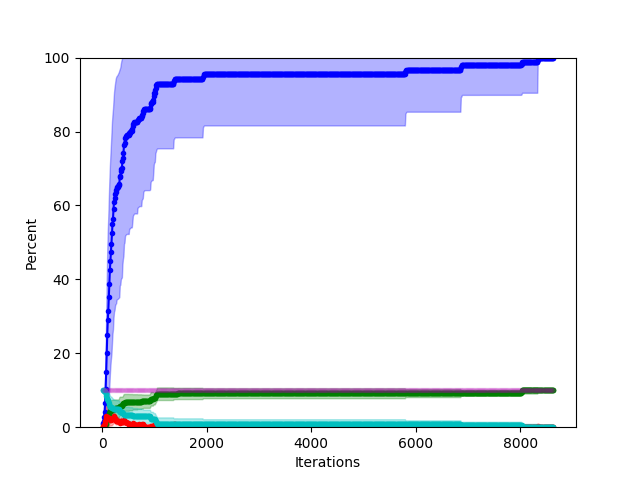
\includegraphics[width=0.329\linewidth]{Network_rA_10.0/new_plots/50.png}
%\caption{Simulation with random nodes, 10\% malicious and range of 10m, 30m and 50m.} 
%\label{fig:random103050}
%\end{figure*}

%\begin{figure}
%\centering
%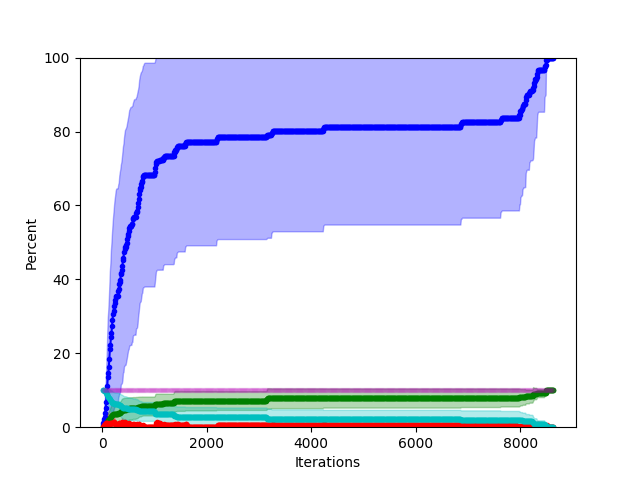
\includegraphics[width=0.5\linewidth]{Network_rA_10.0/new_plots/30.png}
%\caption{Simulation with random nodes and range of 30m.} \label{fig:random30}
%\end{figure}
%
%\begin{figure}
%\centering
%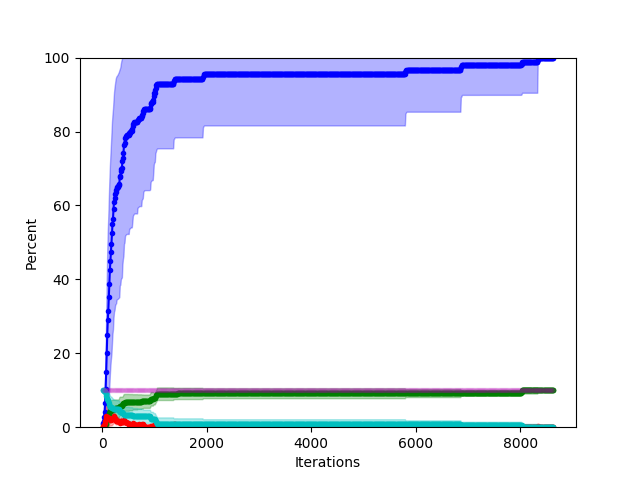
\includegraphics[width=0.5\linewidth]{Network_rA_10.0/new_plots/50.png}
%\caption{Simulation with random nodes and range of 50m.} \label{fig:random50}
%\end{figure}

% ----



%\begin{figure*}
%\centering
%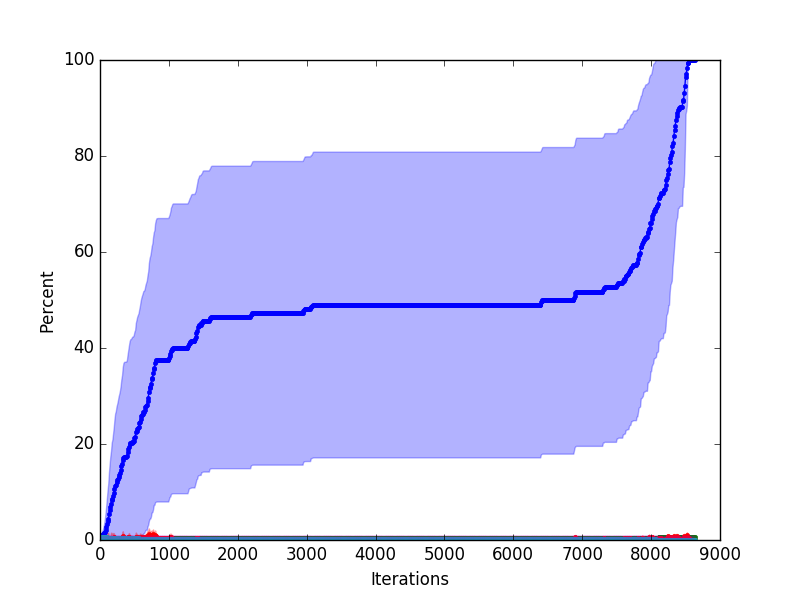
\includegraphics[width=0.329\linewidth]{Network_rA/10_1}
%%\hspace{1pt}
%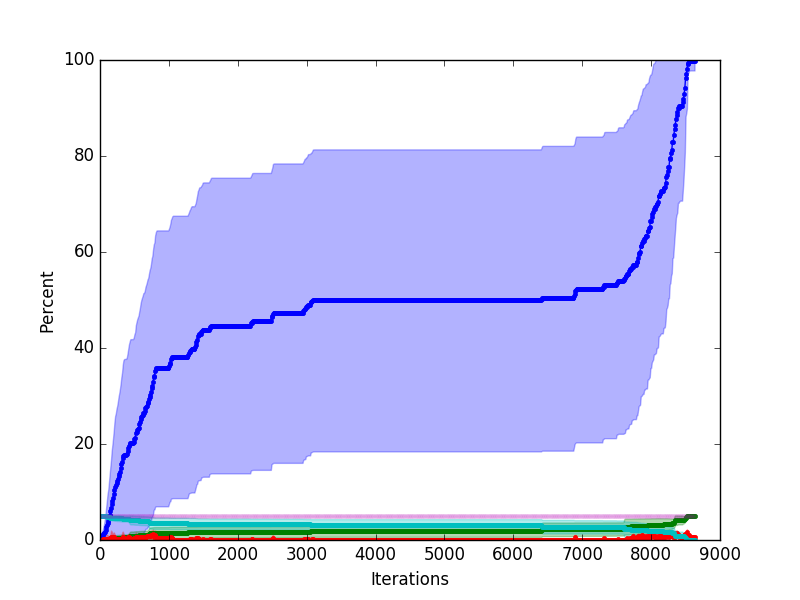
\includegraphics[width=0.329\linewidth]{Network_rA/10_5}
%%\hspace{1pt}
%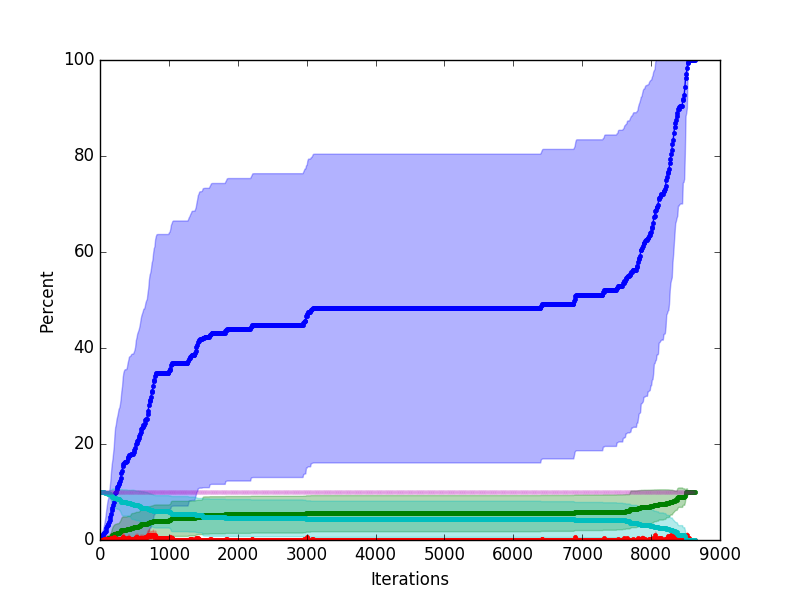
\includegraphics[width=0.329\linewidth]{Network_rA/10_10}
%\caption{Simulation with random nodes, range of 10m and 1\%, 5\% or 10\% malicious.}
%\label{fig:random0}
%\end{figure*}

%\begin{figure}
%\centering0.5
%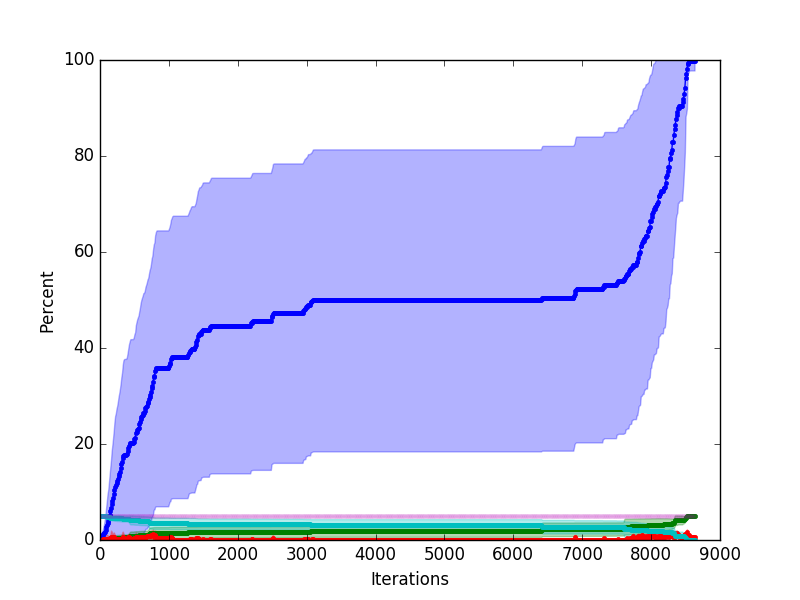
\includegraphics[width=0.5\linewidth]{Network_rA/10_5}
%\caption{Simulation with random nodes, range of 10m and 5\% malicious.} \label{fig:random1}
%\end{figure}
%
%\begin{figure}
%\centering
%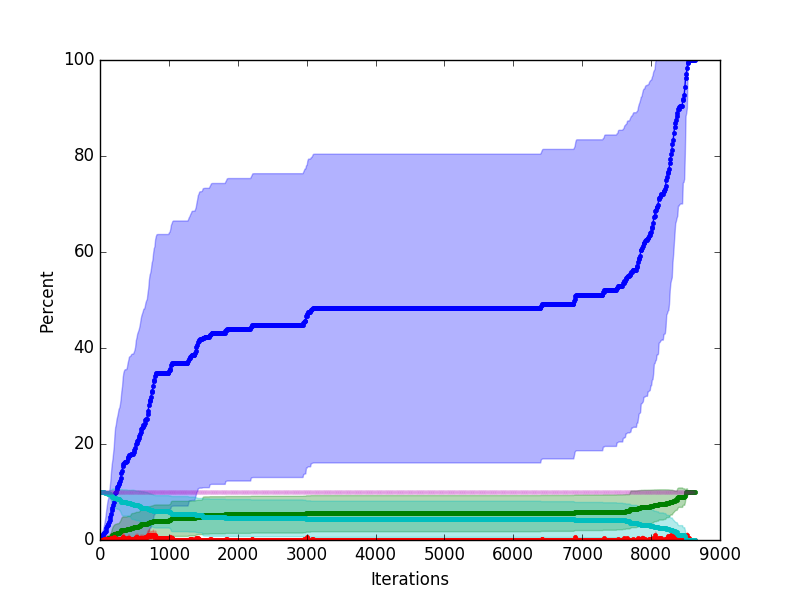
\includegraphics[width=0.5\linewidth]{Network_rA/10_10}
%\caption{Simulation with random nodes, range of 10m and 10\% malicious.} \label{fig:random2}
%\end{figure}

%\begin{figure}
%\centering
%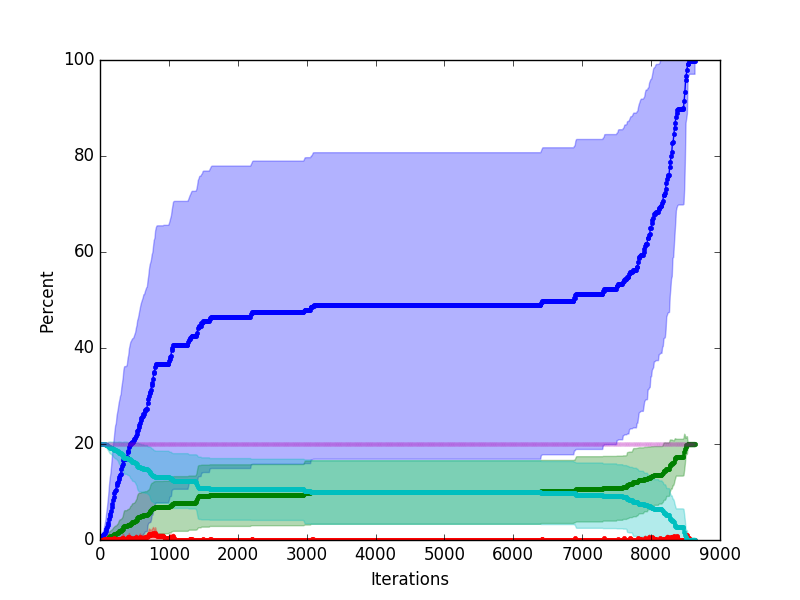
\includegraphics[width=0.5\linewidth]{Network_rA/10_20}
%\caption{Simulation with random nodes, range of 10m and 20\% malicious.} \label{fig:random3}
%\end{figure}

%\begin{figure*}[!t]
%\centering
%\subfloat[]{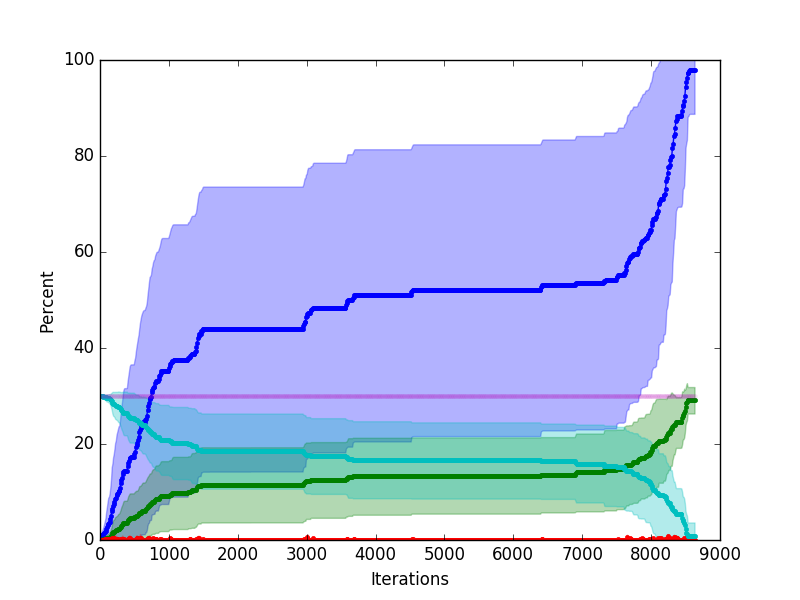
\includegraphics[width=0.329\linewidth]{Network_rA/10_30}%
%\label{subfig:random4}}
%\hfil
%\subfloat[]{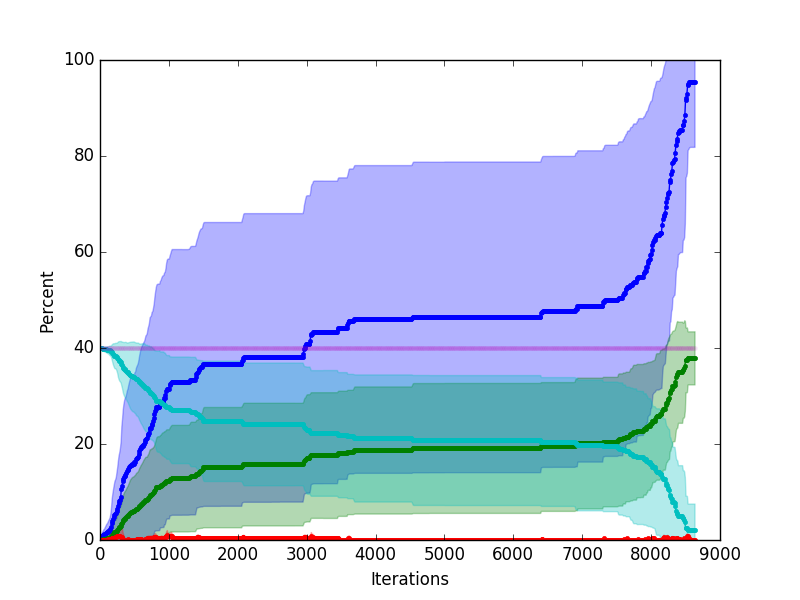
\includegraphics[width=0.329\linewidth]{Network_rA/10_40}%
%\label{subfig:random5}}
%\hfil
%\subfloat[]{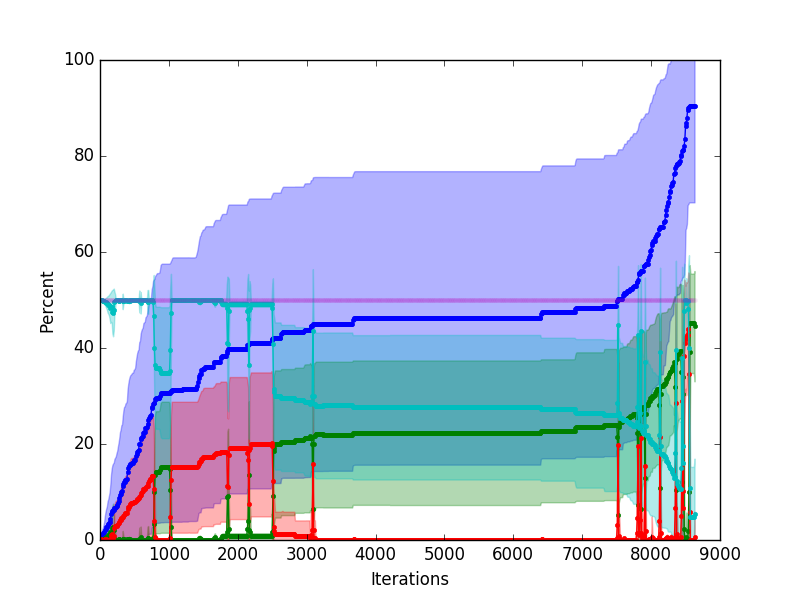
\includegraphics[width=0.329\linewidth]{Network_rA/10_50}%
%\label{subfig:random6}}
%\caption{Simulation with random nodes, range of 10m and (a) 30\%, (b) 40\% or (c) 50\% malicious.}
%\label{fig:random1}
%\end{figure*}

%\begin{figure*}
%\centering
%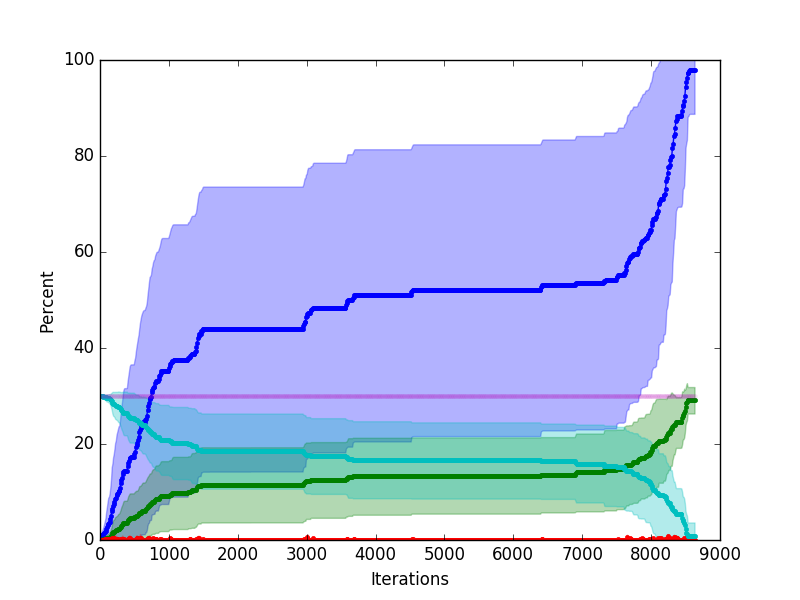
\includegraphics[width=0.329\linewidth]{Network_rA/10_30}
%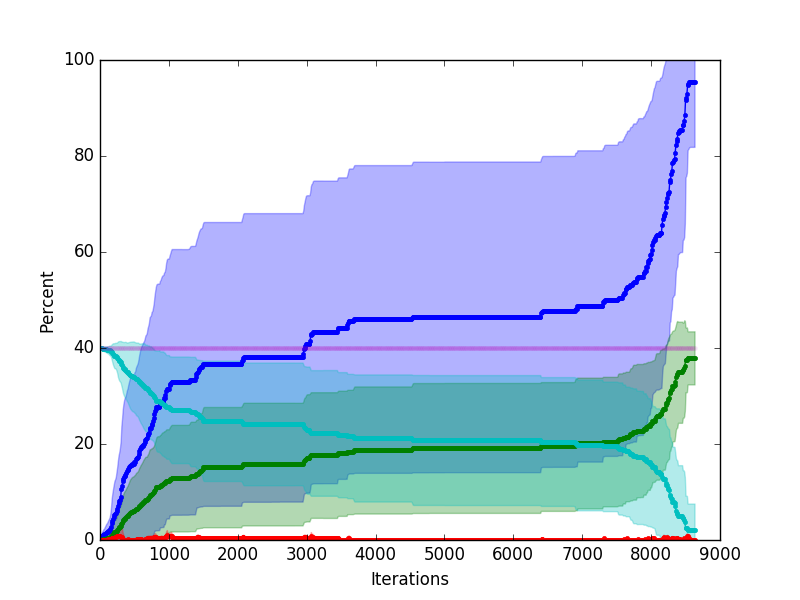
\includegraphics[width=0.329\linewidth]{Network_rA/10_40}
%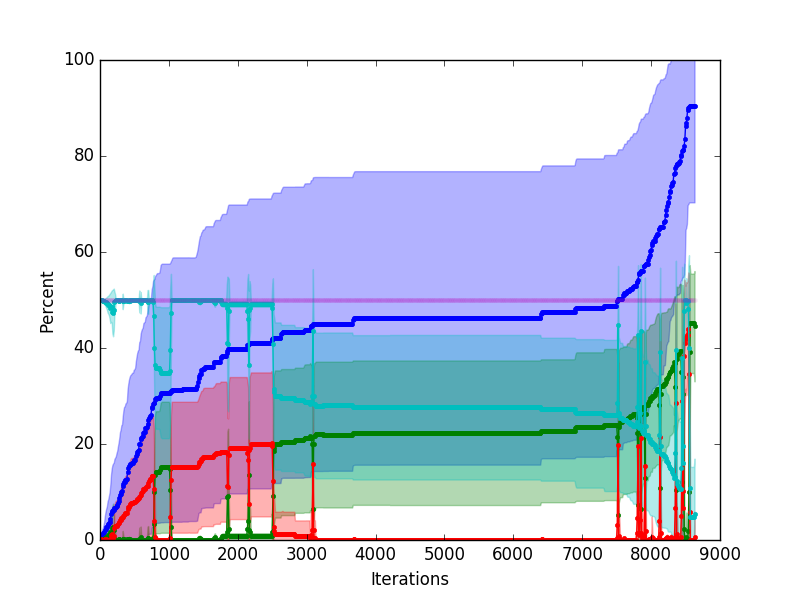
\includegraphics[width=0.329\linewidth]{Network_rA/10_50}
%\caption{Simulation with random nodes, range of 10m and 30\%, 40\% or 50\% malicious.}
%\label{fig:random1}
%\end{figure*}

%\begin{figure}
%\centering
%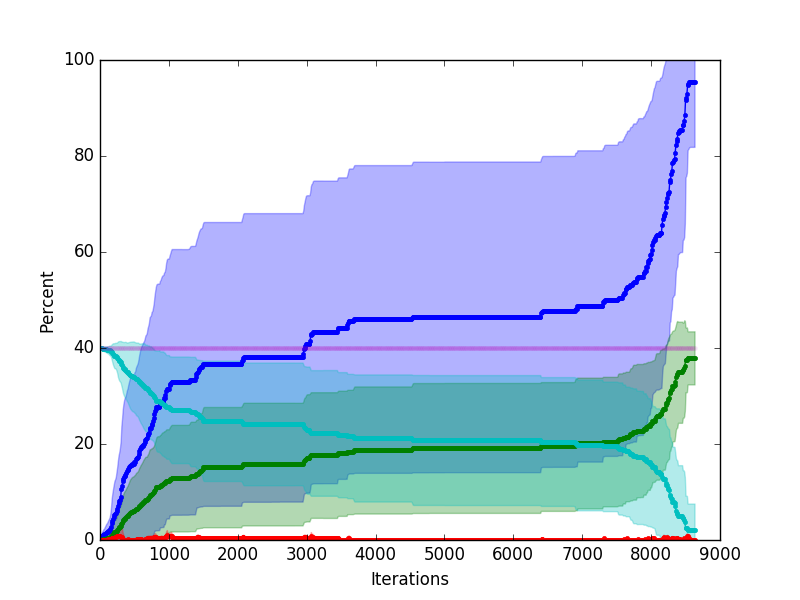
\includegraphics[width=0.5\linewidth]{Network_rA/10_40}
%\caption{Simulation with random nodes, range of 10m and 40\% malicious.} \label{fig:random5}
%\end{figure}
%
%\begin{figure}
%\centering
%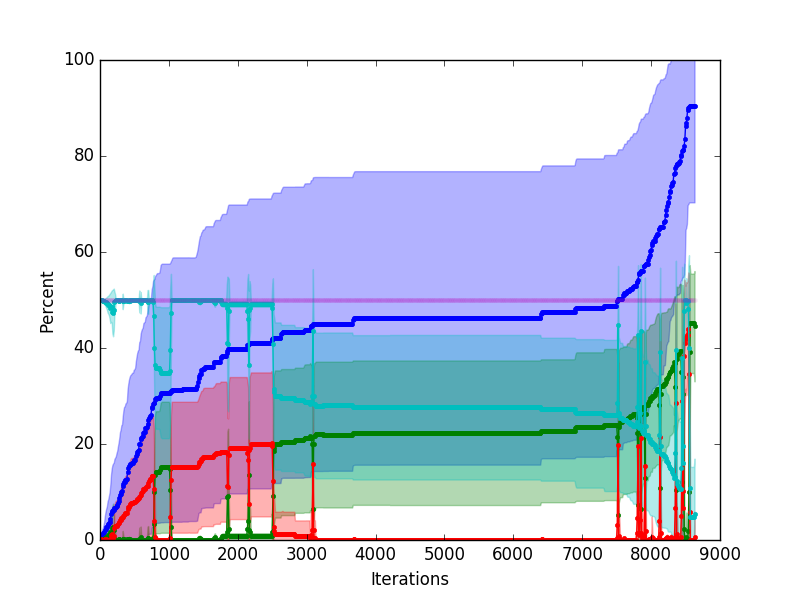
\includegraphics[width=0.5\linewidth]{Network_rA/10_50}
%\caption{Simulation with random nodes, range of 10m and 50\% malicious.} \label{fig:random6}
%\end{figure}

% ----



%\begin{subfigure}{0.20\textwidth}
%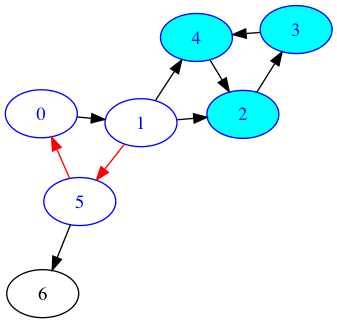
\includegraphics[width=\linewidth]{images/coloring/4.png}
%\caption{Edge $(2,3)$ is checked and node $3$ gets the current value of $d$.} \label{fig:coloring5}
%\end{subfigure}
%\hspace*{2cm} % separation between the subfigures
%\begin{subfigure}{0.20\textwidth}
%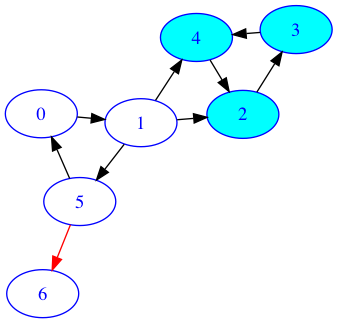
\includegraphics[width=\linewidth]{images/coloring/5.png}
%\caption{Edge $(2,4)$ is checked and node $4$ gets the current value of $d$.} \label{fig:coloring6}
%\end{subfigure}
%\hspace*{2cm} % separation between the subfigures
%\begin{subfigure}{0.20\textwidth}
%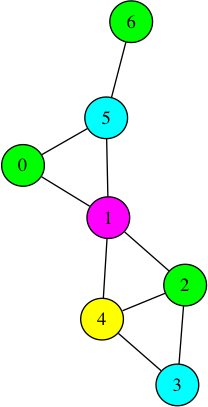
\includegraphics[width=\linewidth]{images/coloring/6.png}
%\caption{Edge $(3,4)$ is checked and node $4$ gets a new color. $d=4$ (yellow).} \label{fig:coloring6}
%\end{subfigure}


% An example of a floating figure using the graphicx package.
% Note that \label must occur AFTER (or within) \caption.
% For figures, \caption should occur after the \includegraphics.
% Note that IEEEtran v1.7 and later has special internal code that
% is designed to preserve the operation of \label within \caption
% even when the captionsoff option is in effect. However, because
% of issues like this, it may be the safest practice to put all your
% \label just after \caption rather than within \caption{}.
%
% Reminder: the "draftcls" or "draftclsnofoot", not "draft", class
% option should be used if it is desired that the figures are to be
% displayed while in draft mode.
%
%\begin{figure}[!t]
%\centering
%\includegraphics[width=2.5in]{myfigure}
% where an .eps filename suffix will be assumed under latex, 
% and a .pdf suffix will be assumed for pdflatex; or what has been declared
% via \DeclareGraphicsExtensions.
%\caption{Simulation results for the network.}
%\label{fig_sim}
%\end{figure}

% Note that the IEEE typically puts floats only at the top, even when this
% results in a large percentage of a column being occupied by floats.


% An example of a double column floating figure using two subfigures.
% (The subfig.sty package must be loaded for this to work.)
% The subfigure \label commands are set within each subfloat command,
% and the \label for the overall figure must come after \caption.
% \hfil is used as a separator to get equal spacing.
% Watch out that the combined width of all the subfigures on a 
% line do not exceed the text width or a line break will occur.
%
%\begin{figure*}[!t]
%\centering
%\subfloat[Case I]{\includegraphics[width=2.5in]{box}%
%\label{fig_first_case}}
%\hfil
%\subfloat[Case II]{\includegraphics[width=2.5in]{box}%
%\label{fig_second_case}}
%\caption{Simulation results for the network.}
%\label{fig_sim}
%\end{figure*}
%
% Note that often IEEE papers with subfigures do not employ subfigure
% captions (using the optional argument to \subfloat[]), but instead will
% reference/describe all of them (a), (b), etc., within the main caption.
% Be aware that for subfig.sty to generate the (a), (b), etc., subfigure
% labels, the optional argument to \subfloat must be present. If a
% subcaption is not desired, just leave its contents blank,
% e.g., \subfloat[].


% An example of a floating table. Note that, for IEEE style tables, the
% \caption command should come BEFORE the table and, given that table
% captions serve much like titles, are usually capitalized except for words
% such as a, an, and, as, at, but, by, for, in, nor, of, on, or, the, to
% and up, which are usually not capitalized unless they are the first or
% last word of the caption. Table text will default to \footnotesize as
% the IEEE normally uses this smaller font for tables.
% The \label must come after \caption as always.
%
%\begin{table}[!t]
%% increase table row spacing, adjust to taste
%\renewcommand{\arraystretch}{1.3}
% if using array.sty, it might be a good idea to tweak the value of
% \extrarowheight as needed to properly center the text within the cells
%\caption{An Example of a Table}
%\label{table_example}
%\centering
%% Some packages, such as MDW tools, offer better commands for making tables
%% than the plain LaTeX2e tabular which is used here.
%\begin{tabular}{|c||c|}
%\hline
%One & Two\\
%\hline
%Three & Four\\
%\hline
%\end{tabular}
%\end{table}


% Note that the IEEE does not put floats in the very first column
% - or typically anywhere on the first page for that matter. Also,
% in-text middle ("here") positioning is typically not used, but it
% is allowed and encouraged for Computer Society conferences (but
% not Computer Society journals). Most IEEE journals/conferences use
% top floats exclusively. 
% Note that, LaTeX2e, unlike IEEE journals/conferences, places
% footnotes above bottom floats. This can be corrected via the
% \fnbelowfloat command of the stfloats package.




\section{Related work}
\label{section:previouswork}

Several models have been proposed to solve the problem of trust in vehicular networks. 
This analysis of related work is based on \cite{zhang2011survey}, which proposes eight desired properties for a trust management model for VANETs.
In the first part of this section, these properties are described with an assessment of whether or not TruMan satisfies their conditions.
Then, some of the most relevant models are described, considering how well they satisfy the desired properties.
\autoref{table:properties} shows how they compare with TruMan.

\begin{figure}
\centering
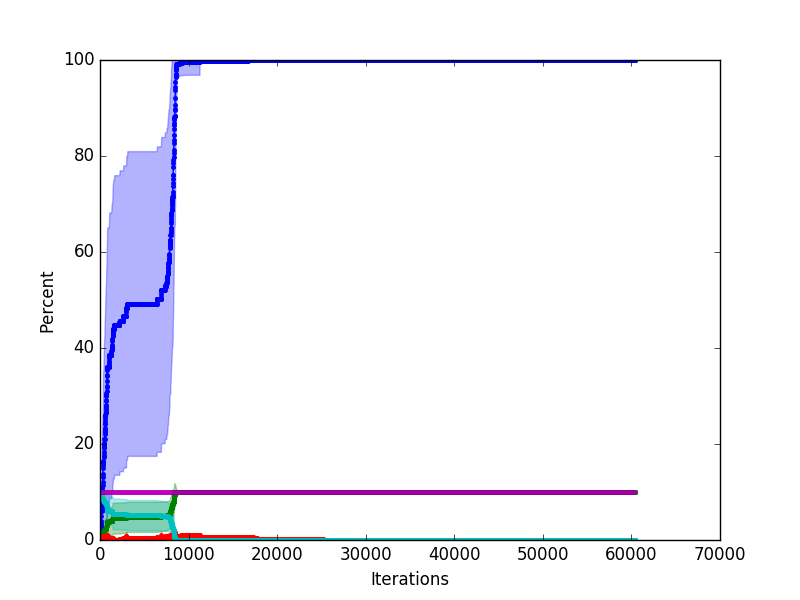
\includegraphics[width=0.5\textwidth]{Network_rA7/10_10}
\caption{7 days scenario: 10m range and 10\% malicious nodes.} \label{fig:random7}
\end{figure}

\subsection{Properties}
\label{section:properties}

\textit{Decentralized trust establishment}: nodes must be able to form their own trust values about other nodes.
Nodes may or may not use information from other trustworthy nodes to build trust values.
TruMan satisfies this as it is built from the ground up for decentralized systems.

\textit{Coping with sparsity}: the model still functions when there are few nodes populating the network.
The experiments using low density values demonstrate that TruMan works in reasonably sparse networks.
Due to its decentralized nature, it can also work on isolated chunks of the network.

\textit{Event/task and location/time dynamics}: how the model reacts to different situations depending on what, where and when events happen.
Although this has not been used in the simulations in this paper, TruMan can easily be extended to consider time and location as long as nodes store geolocation and timestamp data.

\textit{Scalability}: the model can work on very large networks at high speeds.
Due to the low complexity of the algorithms used in the model, TruMan can be highly scalable, as it does not incur substantial pressure on the vehicles' on-board units.
It has also been demonstrated that iterations of the algorithm do not need to run extremely frequently in order to detect malicious nodes with high accuracy.

\textit{Integrated confidence measure}: allows nodes to estimate how useful the output of the algorithm is.
Since nodes using TruMan store trust values as a number between 0 and 1, this value can be used as a confidence measure of the opinion.
The closer it is to 1, the higher the chance that it is accurate.

\textit{System level security}: requires authentication of nodes participating in the network.
This has not been considered in evaluations of TruMan.
However, it can be included as a separate security model during the transmission of messages.

\textit{Sensitivity to privacy concerns}: avoids eavesdropping and stalking by malicious nodes.
TruMan has not been designed with this in mind, but it does not inhibit privacy protection.
However, it does require that nodes cannot be completely anonymous.

\textit{Robustness}: the model's resistance to attacks.
TruMan satisfies this property. Malicious nodes are quickly and accurately identified, making it difficult for them to perform attacks.
Experiments show that, when fewer than 50\% of nodes in the network are malicious, Truman performs as expected.
Collusion attacks must be performed by more than half of the entire network, in which case the network is considered compromised.
Furthermore, since nodes take into consideration experiences from other trustworthy nodes, a malicious node that occasionally behaves correctly can still be identified. 

\subsection{Comparison with other trust models}
\label{section:comparison}

For the Malicious Node Identification Algorithm (MaNI) proposed in \cite{vernize2015malicious}, the authors present a malicious node identification scheme based on strongly connected components and graph coloring.
The model is proposed for complex networks in general, but it is designed only for static networks and the algorithm relies on a global observer which has information about the complete network.
It is, however, very efficient thanks to the classification of nodes into components and the usage of a fast heuristic.
The usage of strongly connected components and coloring serves as a basis for TruMan, which is expanded to work on distributed and dynamic networks such as vehicular networks.

The model proposed in \cite{minhas2010towards} uses several criteria to judge whether or not a received message is trustworthy.
First, nodes are classified by their roles, used for vehicles which should be automatically trustworthy (i.e. police cars).
Nodes also store their experience each time an event message is received (if one neighboring node reported an event which did not turn out to be true, its trust value is reduced).
Additionally, messages have higher reliability when their senders are closer in time and space to the reported event.
When several messages about the same event are received, a node can either choose the $n$ most trustworthy senders, according to the priority (fewer chosen nodes mean a faster, but less precise, decision), or compute the majority opinion of the messages according to each sender's trust value.
%The model considers both role-based trust and experience-based trust; although the work proposed here does not use role-based trust, the authors provide a useful method of calculating and updating an experience-based trust value, which might be used or adapted.
However, the model relies only on direct interaction between pairs of nodes, so no form of indirect trust is considered.

In \cite{chen2010trust}, the authors propose to evaluate messages utilizing a cluster-based trust model.
By separating nodes into clusters with their geographical neighbors, it is possible to distribute the evaluation of messages using previously formed opinions.
When a node sends a message, the cluster-leader must aggregate the other nodes' opinions on that message.
Messages are only forwarded to other clusters if the aggregate opinion is above a certain threshold. Additionally, nodes that receive the message only act if the overall trust on it is above another threshold.
However, it is unclear how the model behaves when the network is too sparse to form relevant clusters, neither do the authors inform how the aforementioned thresholds are decided.
Furthermore, maintaining clusters in a highly dynamic network is a costly job and, if the cluster leader itself is malicious, all the information from that cluster become untrustworthy.

The ART model proposed in \cite{li2016art} works in two main steps: data gathering and malicious node detection.
It uses the Dempster-Shafter theory of evidence to merge data coming from other nodes.
Then, it uses a Cosine-based metric to compare two nodes' trust vectors (a series of opinions regarding other nodes).
However, these steps require several intensive calculations, which greatly increase the complexity of the algorithm.
The authors present no details on how it deals with sparsity, dynamics, scalability, security and privacy.

The authors of \cite{chen2017cloud} propose a cloud-based solution for a trust model, which requires an Internet-based global trust manager.
This has the advantage of simplifying properties such as handling sparsity and scalability, but also makes the system slower in general, especially in situations in which mobile communication is slow or unreliable.
It also makes the system prone to attacks, since the whole system collapses if the global trust manager is attacked.

Finally, it is worth noting that, aside from \cite{vernize2015malicious}, none of the mentioned related work presents complexity calculations for their algorithm.
Considering the scale of the problem, TruMan's cost of $O(|V|\times |E|)$ is very low without sacrificing completeness and correctness.
The model still satisfies or permits most of the desired properties of a trust model, making it viable for real-world use.

%None of them provide a complete solution, but serve as pieces of a puzzle that is still incomplete. 
%Many trust management solutions for VANETs have been proposed over the years, such as \cite{patwardhan2006data}, \cite{gerlach2007trust}, \cite{raya2008data}, \cite{huang2010situation}, \cite{ding2013novel}, \cite{haddadou2013trust}, \cite{liu2016lsot}, \cite{kerrache2016detection}.
%There are also some review and/or survey articles on the subject of VANET trust models, such as \cite{zhang2011survey}, \cite{ma2011survey}, \cite{zhang2012trust}, \cite{mejri2014survey}, \cite{soleymani2015trust} \cite{sengar2016survey}, and \cite{dwivedi2016review}.
%


\begin{table}[t!]
\caption{Properties of Truman and related work}
\label{table:properties}
\centering
\begin{tabular}{|p{1.5cm}||p{1.1cm}|p{1.1cm}|p{0.4cm}|p{0.4cm}|p{0.4cm}|p{0.4cm}|p{0.4cm}|}
 \hline
 \textbf{Property} & Truman & \cite{vernize2015malicious} & \cite{minhas2010towards} & \cite{chen2010trust} & \cite{li2016art} & \cite{chen2017cloud} \\
 \hline
 Decentralized 	& \checkmark & -		  & \checkmark & \checkmark & \checkmark & - \\
 \hline
 Sparsity 		& \checkmark & -		  & \checkmark & \checkmark & -			 & \checkmark \\
 \hline
 Dynamics 		& \checkmark & - 		  & \checkmark & \checkmark & -			 & - \\
 \hline
 Scalability 	& \checkmark & \checkmark & \checkmark & \checkmark & -			 & \checkmark \\
 \hline
 Confidence 	& \checkmark & \checkmark & \checkmark & \checkmark & \checkmark & - \\
 \hline
 Security 		& -			 & - 		  & \checkmark & \checkmark & - 		 & \checkmark \\
 \hline
 Privacy 		& - 		 & - 		  & \checkmark & - 			& -			 & \checkmark \\
 \hline
 Robustness 	& \checkmark & -		  & -		   & - 			& \checkmark & - \\
 \hline
 Efficiency		& \checkmark & \checkmark & -		   & -			& -			 & - \\
 \hline
 Cost & $|V|*|E|$ & $|V|+|E|$ & n/a & n/a & n/a & n/a\\
 \hline
% \hline
\end{tabular}
\end{table}


\section{Conclusion}
\label{section:conclusion}

The concept of trust as applied in VANETs is a powerful tool for those seeking to reduce the spread of false information as much as possible.
In this paper, a new trust model for vehicular networks was presented, which combines the efficiency of previous algorithms in order to generate fast and accurate results.
As nodes travel across the network and collect more data from neighbors, they are able to form an abstraction of the network which can be used to detect malicious nodes.
By placing nodes into strongly connected components, a network containing a large amount of node can be simplified into a much smaller one.
Using a simple graph coloring algorithm, most malicious nodes stand out by having different colors than the majority of nodes.
This allows for a low complexity approach to malicious node identification in a dynamic network.

The experiments show that vehicles within a network can form a sufficient model of the network in around one day, and by then they are also able to detect nearly every malicious node in the network, with a very tiny amount of false positives.
As the network changes in shape, nodes acquire more information and are able to make even more accurate classifications of malicious nodes around them. Future work includes the extension of the proposed model to use V2I communications.
%Since trust amongst nodes in the network is a value ranging between 0 and 1, the trust between two nodes gradually increases or decreases according to the results of each iteration.

% conference papers do not normally have an appendix


% use section* for acknowledgment
%\section*{Acknowledgment}
%
%
%The authors would like to thank...





% trigger a \newpage just before the given reference
% number - used to balance the columns on the last page
% adjust value as needed - may need to be readjusted if
% the document is modified later
%\IEEEtriggeratref{8}
% The "triggered" command can be changed if desired:
%\IEEEtriggercmd{\enlargethispage{-5in}}

% references section

% can use a bibliography generated by BibTeX as a .bbl file
% BibTeX documentation can be easily obtained at:
% http://mirror.ctan.org/biblio/bibtex/contrib/doc/
% The IEEEtran BibTeX style support page is at:
% http://www.michaelshell.org/tex/ieeetran/bibtex/
\bibliographystyle{IEEEtran}
% argument is your BibTeX string definitions and bibliography database(s)
\bibliography{article}
%
% <OR> manually copy in the resultant .bbl file
% set second argument of \begin to the number of references
% (used to reserve space for the reference number labels box)
%\begin{thebibliography}{1}
%
%\bibitem{IEEEhowto:kopka}
%H.~Kopka and P.~W. Daly, \emph{A Guide to \LaTeX}, 3rd~ed.\hskip 1em plus
%  0.5em minus 0.4em\relax Harlow, England: Addison-Wesley, 1999.
%
%\end{thebibliography}




% that's all folks
\end{document}


